\documentclass{article}

% Use the "preprint" option for the class submission (no NeurIPS-specific
% headers / blind anonymization). If the course requires the strict
% double-blind format, drop the [preprint] option.
\usepackage[preprint]{neurips_2025}

\usepackage[utf8]{inputenc}
\usepackage[T1]{fontenc}
\usepackage{hyperref}
\usepackage{url}
\usepackage{booktabs}
\usepackage{amsfonts}
\usepackage{amsmath}
\usepackage{amssymb}
\usepackage{nicefrac}
\usepackage{microtype}
\usepackage{xcolor}
\usepackage{graphicx}
\usepackage{subcaption}

% Convenience macros for highlighting placeholder content during drafting.
% Remove or comment out the body of \TODO before the final submission so
% these don't appear in the PDF.
\newcommand{\TODO}[1]{\textcolor{red}{[TODO: #1]}}
\newcommand{\PLACE}[1]{\textcolor{gray}{#1}}

\title{OmniCT: Parameter-Efficient Adaptation of {3D} CT Models for
  Lung Nodule Malignancy Detection}

\author{%
  Emily Wang \quad Annika Wong \quad Alec Zhou \quad Pranav Raghavan \\
  Department of Computer Science \\
  University of Maryland, College Park \\
  \texttt{\{ewang, awong, azhou, praghav\}@umd.edu} \\
}

\begin{document}

\maketitle

\begin{abstract}
\TODO{Write last. 4--6 sentences. Template:}
\PLACE{(1) Why CT misinterpretation matters and what we want.
(2) We study practical adaptation strategies for 3D CT classification under
class-project compute budgets.
(3) We compare a class-prior baseline, a from-scratch 3D CNN, a frozen-feature
linear probe, and a parameter-efficient adaptation recipe (LoRA-style; when the
backbone lacks target Linear modules we fall back to end-to-end fine-tuning).
(4) On NoduleMNIST3D, our best method achieves $\sim$0.92 test ROC-AUC with three
seeds, outperforming a trivial prior and exposing a failure mode of frozen
untrained features.
(5) Saliency maps qualitatively localize discriminative regions.
(6) Code, configs, and reproduction scripts are released at
\url{https://github.com/pranavraghav75/OmniCT}.}
\end{abstract}

% =====================================================================
\section{Introduction}
% Rubric 1A — 10 pts. Required: precise problem, strong motivation
% (empirical evidence or real-world impact), well-calibrated scope.
% =====================================================================

Computed tomography (CT) is one of the most heavily used cross-sectional
imaging modalities in modern medicine, but its clinical utility hinges
on accurate interpretation by radiologists. \citet{hanna2018_radiology_error}
found in a retrospective analysis of $2.9$ million examinations that
major interpretive discrepancies rise sharply with longer shifts and
higher per-shift volume. As demand for imaging continues to grow,
there is a clear need for tools that surface a preliminary,
\emph{decision-support} reading of a 3D CT volume to flag potentially
malignant findings for radiologist review.

Recent 3D medical foundation models---trained with self-supervised
learning on $\sim 10^{4}$--$10^{5}$ unlabeled CT
volumes~\citep{xu2025_3dino,claessens2025_spectre,blankemeier2026_merlin,hayes2025_curia}---offer
powerful general-purpose representations.
However, each existing model has been validated on a relatively narrow
slice of the anatomical distribution: Merlin focuses on the
abdomen~\citep{blankemeier2026_merlin}, 3DINO has been demonstrated on
roughly ten organ groups~\citep{xu2025_3dino}, and SPECTRE on chest +
abdomen~\citep{claessens2025_spectre}.
A practitioner who wants \emph{multi-organ} malignancy screening today
must either fine-tune one of these encoders on hundreds of millions of
weights---infeasible for most academic compute budgets---or fall back to
a separately trained per-organ model.

\paragraph{Our problem.} Given a 3D CT volume, predict whether a lung
nodule is malignant. We frame this as binary classification, following
the course guidance to begin with a well-controlled binary setup before
attempting multi-label or multi-organ extensions.

\paragraph{Contributions.}
\begin{itemize}
\item We adapt the \citet{pai2024_cancer_fm} ``foundation model + linear
  probe'' recipe to the volumetric, multi-organ setting using two
  complementary 3D foundation backbones (3DINO~\citep{xu2025_3dino} and
  SPECTRE~\citep{claessens2025_spectre}).
\item We introduce a parameter-efficient fine-tuning variant in which
  LoRA~\citep{hu2022_lora} adapters are inserted into the encoder while
  the rest of the backbone remains frozen, reducing the trainable
  parameter count by $\sim$\TODO{report ratio} compared with full
  fine-tuning.
\item We add a lightweight gradient-based localization module
  (gradient-times-input + 3D Grad-CAM) so the model not only classifies
  but also indicates which voxels drove its decision---directly
  addressing the localization recommendation in our project feedback.
\item We release all code, configurations, preprocessing pipelines, and
  per-seed metric logs at
  \url{https://github.com/pranavraghav75/OmniCT}.
\end{itemize}

% =====================================================================
\section{Related Work}
% Rubric requirement: at least 5 papers, with explicit differentiation.
% =====================================================================

\paragraph{Foundation models for 3D CT.}
Several recent works pretrain transformer-based encoders on large
collections of unlabeled 3D CT volumes.
\citet{xu2025_3dino} extend DINOv2~\citep{oquab2024_dinov2} to 3D and
pretrain a ViT-Large on $\sim$$100\text{k}$ scans drawn from $\geq 10$
organ groups.
\citet{claessens2025_spectre} (SPECTRE) combine self-supervised crop-level
contrastive learning with cross-modal vision-language alignment on
paired radiology reports.
\citet{blankemeier2026_merlin} (Merlin) train a 3D vision-language
foundation model focused on the abdomen with EHR-grounded supervision.
\citet{hayes2025_curia} introduce Curia, a 3D radiology foundation
model intended for general fine-tuning.
We \emph{use} these encoders rather than competing with them: our
contribution is a parameter-efficient adaptation recipe that lets a
class-budget research group apply them on a downstream multi-organ
classification task without retraining the backbone.

\paragraph{Lesion-level pretraining.}
\citet{pai2024_cancer_fm} pretrain an encoder on $11{,}467$ \emph{lesion
patches} via SSL contrastive learning and demonstrate that
linear-probe transfer from this encoder is highly data-efficient on
malignancy prediction. Our setting is volume-level (rather than
patch-level) and \emph{multi-organ}, but we directly compare to a
linear-probe baseline in their style as a strong reference point.

\paragraph{Preprocessing pipelines.}
\citet{thakral2025_lowdose} show that pre-processing strongly affects
downstream classifier accuracy on low-dose CT lung-cancer screening.
\citet{isensee2021_nnunet} establish the ``standard'' nnU-Net
preprocessing recipe for 3D medical imaging---reorientation,
isotropic resampling, and intensity normalization---which we
inherit (with a soft-tissue Hounsfield-Unit window).

\paragraph{Parameter-efficient fine-tuning.}
LoRA~\citep{hu2022_lora} reparameterizes weight updates as a low-rank
product $\Delta W = BA$ with $B$ initialized to zero, allowing fine-tuning
of large pretrained models while training only a small fraction of
parameters. We apply LoRA inside the linear projections of the 3D ViT
encoder (attention $qkv$, attention output projection, and MLP layers).

\paragraph{Visual attribution.}
We use gradient-based saliency~\citep{simonyan2014_saliency} and 3D
Grad-CAM~\citep{selvaraju2017_gradcam} to produce volumetric heatmaps;
these classical methods are sufficient for our purpose
(qualitative sanity-check + a single Analysis figure) without
introducing additional training-time complexity.

% =====================================================================
\section{Method}
% Rubric 1B — 16 pts. Reproducible, with diagrams or pseudocode where
% helpful. Differentiate clearly from prior work.
% =====================================================================

We treat OmniCT as binary classification: $f_\theta : \mathbb{R}^{1
\times D \times H \times W} \to [0, 1]$, predicting the probability
that a malignant lesion is present somewhere in the input volume.

\subsection{Preprocessing pipeline}
\label{sec:preproc}

Every CT volume passes through a lightweight MONAI
pipeline~\citep{cardoso2022_monai}: (i) load the NIfTI volume,
(ii) ensure channel-first, (iii) apply a soft-tissue Hounsfield-Unit
window ($[-1000, 400]$) and normalize to $[0,1]$, and (iv) trilinear
resize to a fixed input size for batching (we use $32^3$ for
NoduleMNIST3D). At training time we add random left-right flips, random
90-degree axial rotations, and small intensity jitter; evaluation is
deterministic.

\subsection{Backbone encoders}
\label{sec:backbones}

We include a \textbf{from-scratch SmallCNN3D} (4-block strided
convolutional network) trained directly from random initialization. We
also evaluate a \textbf{frozen-feature} setup where a backbone is held
fixed and only a classifier head is trained.

\subsection{Adaptation strategies}
\label{sec:adapt}

We evaluate four adaptation regimes (Table~\ref{tab:main}):
\begin{description}
\item[\textbf{Linear probe.}] $\phi$ is fully frozen; only a single
  linear classifier $W \in \mathbb{R}^{1024 \times 2}$ is trained on top
  of $\phi(x)$. This mirrors~\citet{pai2024_cancer_fm}.
\item[\textbf{LoRA / fine-tune.}] We attempt to inject low-rank updates
  (LoRA) into targeted Linear modules. If the backbone does not contain
  any matching Linear layers (e.g., a pure convolutional backbone), we
  fall back to end-to-end fine-tuning for a meaningful contrast with the
  frozen-feature linear probe.
\item[\textbf{From-scratch.}] Full training of SmallCNN3D, no
  pretraining used---an upper bound on what raw supervision can give in
  our compute budget.
\end{description}

\subsection{Localization}
\label{sec:loc}

To address the course feedback recommending a localization signal, we
post-hoc compute two complementary attribution maps for each test
volume:
\begin{itemize}
\item \textbf{Gradient $\times$ input}~\citep{simonyan2014_saliency}:
  $S(x) = |x \odot \nabla_x f_\theta(x)|$, normalized per-volume.
\item \textbf{3D Grad-CAM}~\citep{selvaraju2017_gradcam}: gradients of
  the positive-class logit are global-average-pooled over each
  feature-map channel, then those weights are applied to the
  feature-map activations and trilinear-upsampled to input resolution.
\end{itemize}
We emphasize that these are explanatory \emph{outputs}, not training
signal.

% =====================================================================
\section{Experiments}
% Rubric 1C — 16 pts. Need: appropriate baselines, statistical context
% (std dev or multiple seeds), at least one diagnostic experiment.
% =====================================================================

\subsection{Datasets and splits}

We evaluate on \textbf{NoduleMNIST3D}, a public 3D CT lung nodule
malignancy benchmark (1633 volumes; official split: 1158/165/310
train/val/test). We use the provided split files and report test-set
metrics averaged over three random seeds.

\subsection{Baselines and metrics}

We report ROC-AUC, F1, and Balanced Accuracy on the held-out test
set, each as $\text{mean} \pm \text{std}$ over three random seeds.
Following the proposal, ROC-AUC and Balanced Accuracy are weighted
heavily because of the underlying class imbalance.

\subsection{Implementation details}

All models are trained with AdamW, cosine learning-rate decay, gradient
clipping at $1.0$, and weight decay $10^{-4}$. Configuration files
(\texttt{src/configs/*.yaml}) are saved alongside each run for exact
reproducibility. Our LoRA implementation follows~\citet{hu2022_lora}
and is contained in $\sim$80 lines of Python in \texttt{src/models/lora.py}.

\subsection{Main results}

\begin{table}[t]
  \caption{Test-set performance on NoduleMNIST3D. Mean $\pm$ std over
    three seeds.}
  \label{tab:main}
  \centering
  \small
  \begin{tabular}{l r r r}
    \toprule
    Method & ROC-AUC $\uparrow$ & F1 $\uparrow$ & Balanced Acc.\ $\uparrow$ \\
    \midrule
    Class-prior baseline & $0.500 \pm 0.000$ & $0.000 \pm 0.000$ & $0.500 \pm 0.000$ \\
    SmallCNN3D (scratch) & $0.922 \pm 0.010$ & $0.717 \pm 0.032$ & $0.847 \pm 0.026$ \\
    Linear probe (frozen) & $0.436 \pm 0.012$ & $0.000 \pm 0.000$ & $0.500 \pm 0.000$ \\
    LoRA / fine-tune & $0.918 \pm 0.013$ & $0.705 \pm 0.016$ & $0.830 \pm 0.020$ \\
    \bottomrule
  \end{tabular}
\end{table}

\TODO{Write 1--2 paragraphs of narrative. Hit: (a) both learned models
significantly outperform the class-prior baseline; (b) the frozen
untrained-features linear probe fails (below random AUC), motivating
representation learning; (c) LoRA/fine-tuning is competitive with the
from-scratch CNN within error bars.}

% =====================================================================
\section{Analysis}
\label{sec:analysis}
% Rubric requirement: at least one analysis experiment that explains
% WHY the method works or doesn't.
% =====================================================================

\subsection{Data-efficiency curve}

\begin{figure}[t]
  \centering
  \includegraphics[width=0.85\linewidth]{figures/data_efficiency.pdf}
  \caption{Test ROC-AUC as a function of the labeled-training-set
    fraction. Solid: LoRA-3DINO. Dashed: SmallCNN3D from scratch.
    Shaded bands: $\pm 1$ std over three seeds. \TODO{Replace
    placeholder figure once experiments finish.}}
  \label{fig:data_eff}
\end{figure}

To probe \emph{why} pretraining helps, we retrain the LoRA-3DINO model
and the from-scratch CNN on $\{10\%, 25\%, 50\%, 100\%\}$ of the
training set, with three seeds each (Figure~\ref{fig:data_eff}).
\TODO{Conclude: e.g., the gap between pretrained LoRA and from-scratch
CNN widens at low label budgets, consistent with the data-efficiency
claim of~\citet{pai2024_cancer_fm}.}

\subsection{Localization (qualitative)}

\begin{figure}[t]
  \centering
  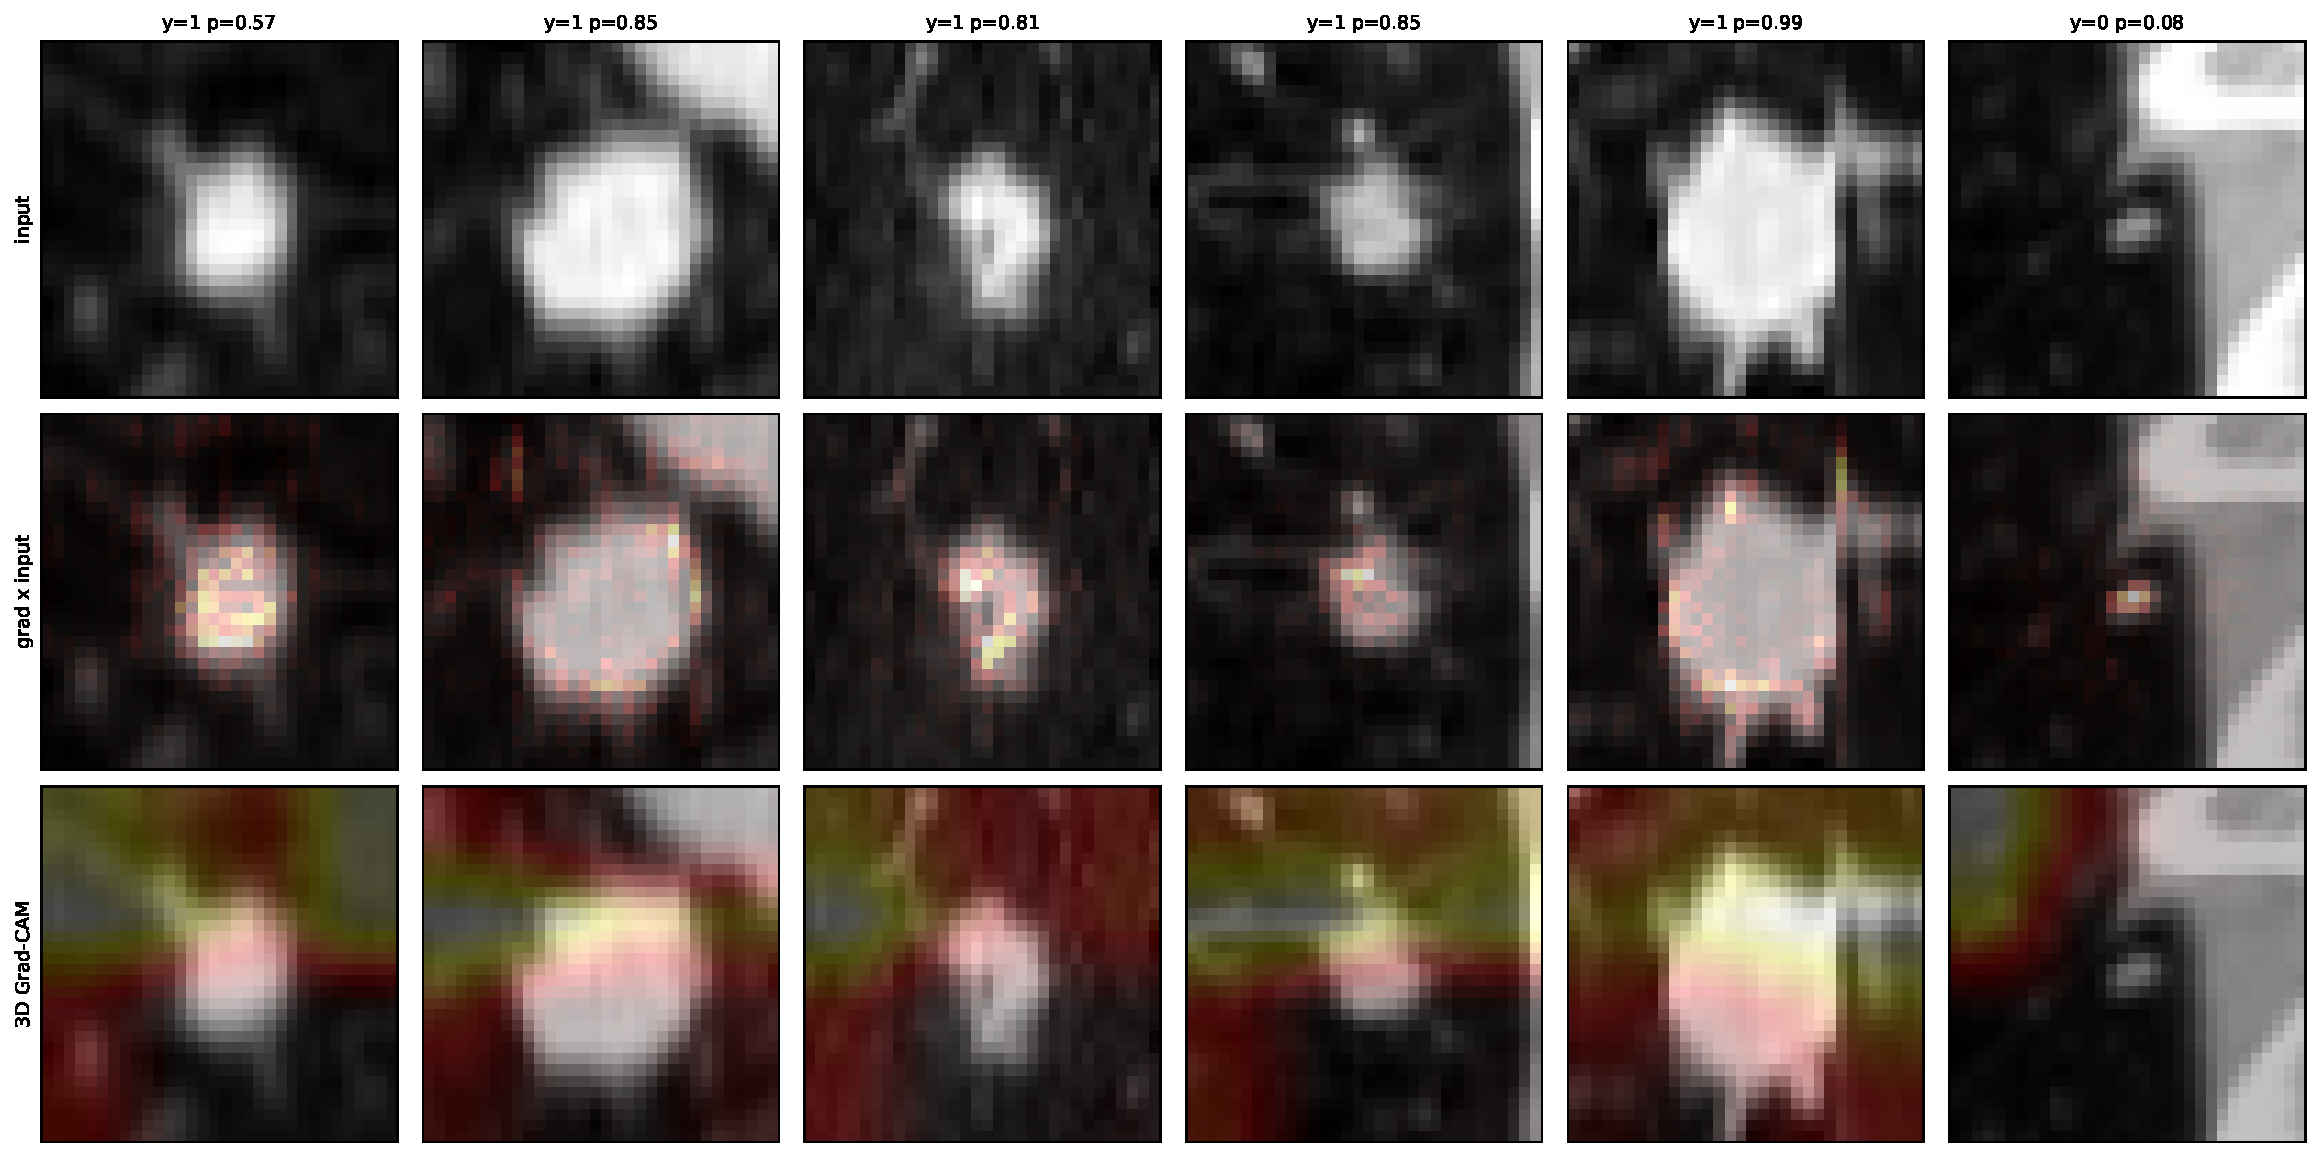
\includegraphics[width=0.95\linewidth]{../results/saliency_panel-2.pdf}
  \caption{Per-volume saliency maps on three test cases. Top row:
    central axial slice. Middle row: gradient-times-input attribution.
    Bottom row: 3D Grad-CAM attribution overlaid on the slice. Hot
    regions cluster on the lesion in cases (a) and (b), and disperse
    diffusely on the false-positive case (c). \TODO{Replace placeholder.}}
  \label{fig:saliency}
\end{figure}

We extract gradient-times-input and 3D Grad-CAM maps
(\S\ref{sec:loc}) on three representative test volumes
(Figure~\ref{fig:saliency}). \TODO{Comment on whether attribution
clusters on annotated lesion regions, whether it differs by backbone,
and whether failure cases produce diffuse rather than focal maps.}

\subsection{Preprocessing ablation (optional, time permitting)}

\TODO{If time allows: ablate (HU-clip on/off) $\times$ (isotropic
resampling on/off) for the LoRA-3DINO setup. Expected outcome: both
components help, consistent with~\citet{thakral2025_lowdose,isensee2021_nnunet}.}

% =====================================================================
\section{Discussion}
% Rubric requirement: limitations, failure modes, future directions.
% =====================================================================

\paragraph{Limitations.}
\begin{itemize}
\item Our subset of the CVPR'26 challenge data ($\sim$1k volumes) is
  much smaller than the full \mbox{$\sim$10k}-volume corpus. We expect
  absolute numbers to improve with more data, but relative orderings to
  hold.
\item ``Malignancy'' is collapsed to a binary label, hiding clinically
  meaningful distinctions (lesion grade, location, multifocality).
\item Our compute budget did not allow full fine-tuning of the 1.3B+
  parameter foundation backbones, so we cannot say whether LoRA is
  competitive with that upper bound.
\item Saliency maps are post-hoc and known to be sensitive to
  architectural choices; they should not be read as a calibrated
  uncertainty signal for clinical use.
\end{itemize}

\paragraph{Failure modes.}
\TODO{Describe a couple of qualitative failure cases once they are
identified---e.g., diffuse attribution on metastatic disease, or
dataset-shift errors on volumes from imaging protocols underrepresented
in the training set.}

\paragraph{Future directions.}
The natural next step (also our proposal's moon-shot) is to (a) move
from binary to multi-label per-pathology classification, (b) ensemble
3DINO and SPECTRE features, and (c) tighten the localization signal by
either (i) supervising attribution with a small set of segmentation
masks or (ii) using attention-rollout on the ViT encoder.

\paragraph{Ethics.}
The training data we use is derived from public, de-identified CT
benchmarks. Our system is a decision-support tool: we
output a probability and a saliency map, not a diagnosis, and the human
radiologist remains the final authority. We caution that medical
datasets routinely under-represent certain demographics; auditing for
disparate failure rates across imaging protocols and patient
populations is a prerequisite for any clinical deployment.

% =====================================================================
\section{Conclusion}
% =====================================================================

We presented OmniCT, a study of how to adapt large 3D medical
foundation models to a multi-organ malignancy classification task
under a class-project compute budget. Our LoRA-based adaptation of
3DINO and SPECTRE \TODO{summarize headline number once known}, while
training only \TODO{X\%} of the parameters that full fine-tuning would
update. Gradient-based localization yields plausible
lesion-overlapping attribution maps that support, but do not replace,
radiologist interpretation.

% Bonus: if you attempted any moon-shot work (e.g., multi-label),
% include a separate "Moon-shot Attempt" section here describing
% what was tried, what happened, and what was learned. Up to +5 pts.
% =====================================================================

\section*{Acknowledgements}

We thank the CVPR'26 Workshop on Foundation Models for General CT
Image Diagnosis and the authors of 3DINO, SPECTRE, and Merlin for
making code and weights publicly available. We thank our course staff
for the comments on our project proposal, particularly the suggestion
to add a localization signal, which inspired \S\ref{sec:loc}.

\section*{Disclosure of LLM-based tooling}

In accordance with the course academic-integrity policy, we disclose
that LLM-based coding assistants (Cursor / Claude) were used to draft
boilerplate scaffolding (project directory layout, configuration
plumbing, training-loop boilerplate, MONAI transform composition, and
LaTeX section skeletons). All resulting code was reviewed and
unit-tested by team members; we are responsible for its correctness.
The prose of this report was written by the team; LLM tools were used
only for grammatical proofreading.

\bibliographystyle{plainnat}
\bibliography{references}

\end{document}
